\section{Wprowadzenie}
%\subsection{Machine learning}
%\subsection{Indukcyjne bazy danych}
%\subsection{Zastosowania}

Integracja technologii baz danych z nowoczesnymi metodami indukcyjnego
generowania wiedzy wydaje si� dawa� istotne korzy�ci w perspektywie
budowy system�w wspomaganie decyzji. Systemy nazywane czasem
indukcyjnymi bazami danych potrafi� odpowiedzie� nie tylko na pytania,
dla kt�rych odpowied� znajduje si� w bazie danych, ale r�wnie� na
pytania, kt�re wymagaj� zsyntetyzowania i zastosowania wiarygodnej
wiedzy, wygenerowanej przez indukcyjne wnioskowanie z fakt�w z bazy
danych i wcze�niejszej wiedzy.  Indukcyjne bazy danych mog� by�
postrzegane jako naturalny krok w rozwoju system�w bazodanowych \cite{bib3}.

\begin{figure}[ht]
    \centering
        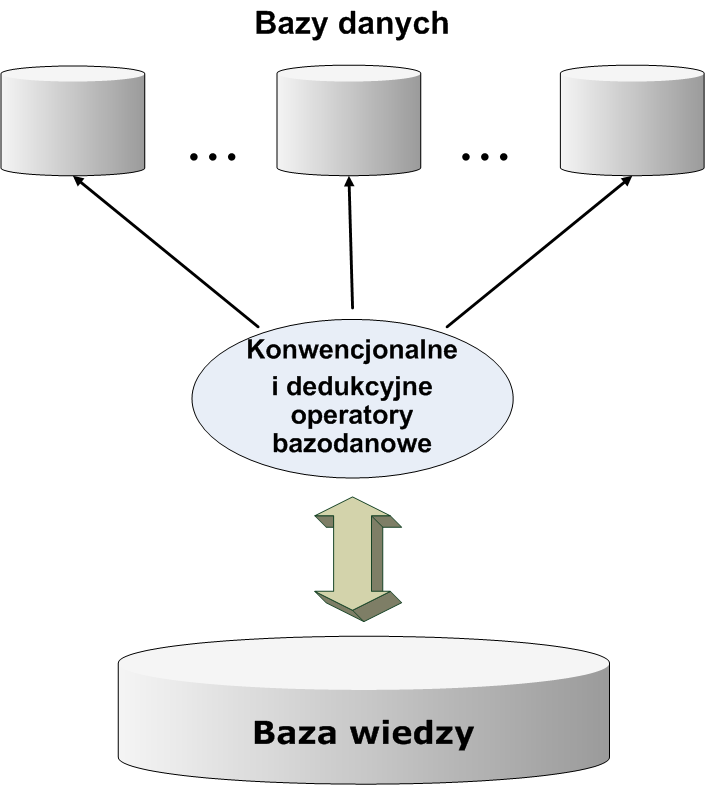
\includegraphics[width=0.70\textwidth]{img/knowledge_mining.png}
    \caption{Indukcyjne bazdy danych}
    \label{fig:architecture}
\end{figure}

\bigskip
W pracy przedstawiona zostanie architektura i wybrane aspekty
implementacji platformy \emph{Salomon}, jak r�wnie� zaprezentowane
zostan� mo�liwo�ci jego wykorzystania na przyk�adzie wybranych
algorytm�w pozyskiwania wiedzy z danych.

%\newpage